\section{Evaluation}
%
% Overview
%

\subsection{Demographic of the Sample}

The following demographic data was drawned out from the pre study survey. Participant's were mostly in their early twenties and mostly males. Out of 27 participants, 2 didn't have a driving license and 25 had a driving license with most of them have been driving for a year. Furthermore 22 participants identified them self as playing videos games, from which 18 participants stated they have played racing video games. The majority of participants who plays racing games identified them self as playing mostly arcade sim racing games, while only 3 play sim racing games. Out of the 27 participants, 7 participants have previously used a racing rig.

%I included the charts in the appendices as I didn't feel like they were adding much over here ending up just taking space.

\begin{figure}[!htb]
	\centering
	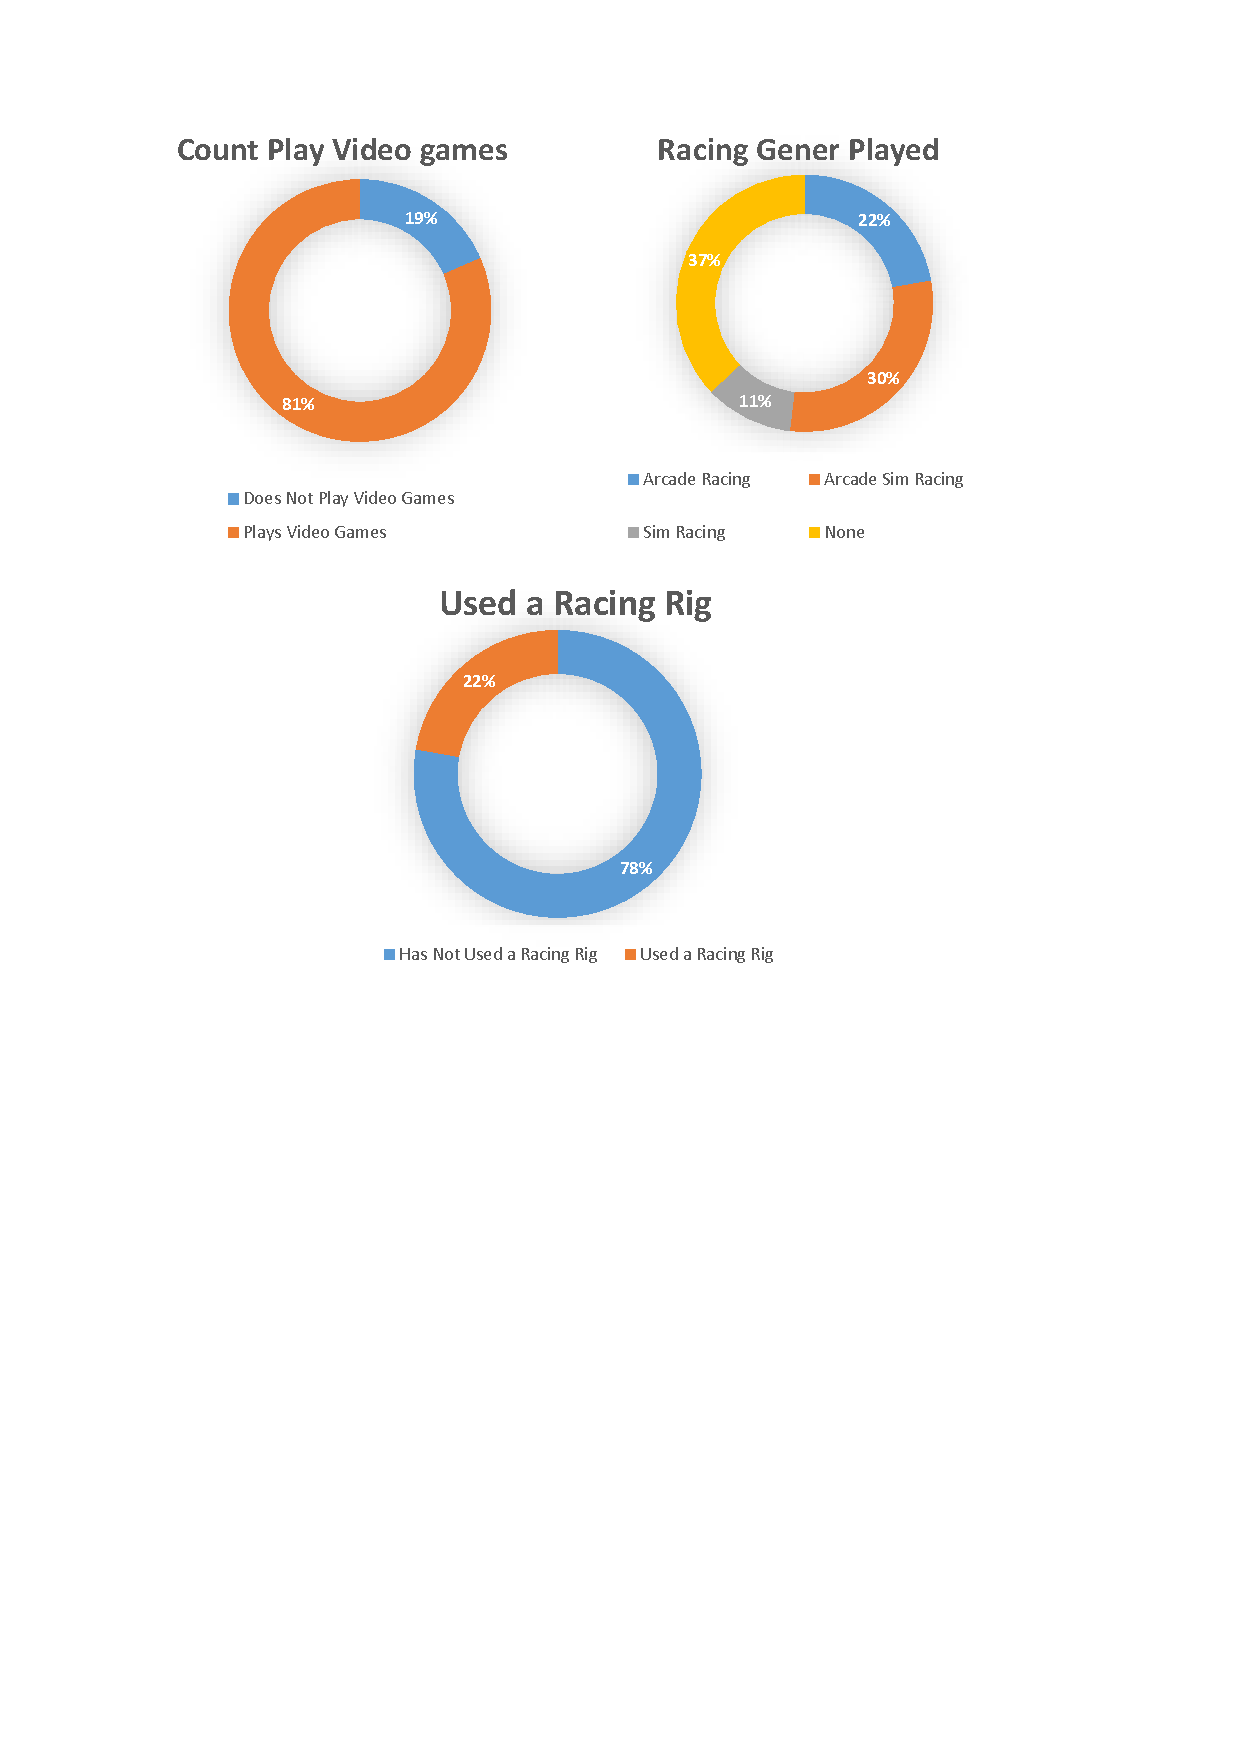
\includegraphics[width=\textwidth]{charts/gamesxp.pdf}
	\caption[Gaming xp]{Video games experience}
	\label{fig:chart-gamesxp}
\end{figure}

\subsection{Distribution tests}

\begin{figure}[!htb]
	\centering
	\includegraphics[width=\textwidth]{charts/laptimes.png}
	\caption{Lap times vs session, clustered by group}
	\label{fig:chart-laptimes}
\end{figure}


Carrying out Shapiro-Wilk test for normality for the feedback group and base group during the first session on their respective lap times it was found that the data is not normally distributed as the p-value for both groups is below 0.05 resulting in rejecting the null hypothesis stating the samples come from a normal distribution

\begin{figure}[!htb]
	\centering
	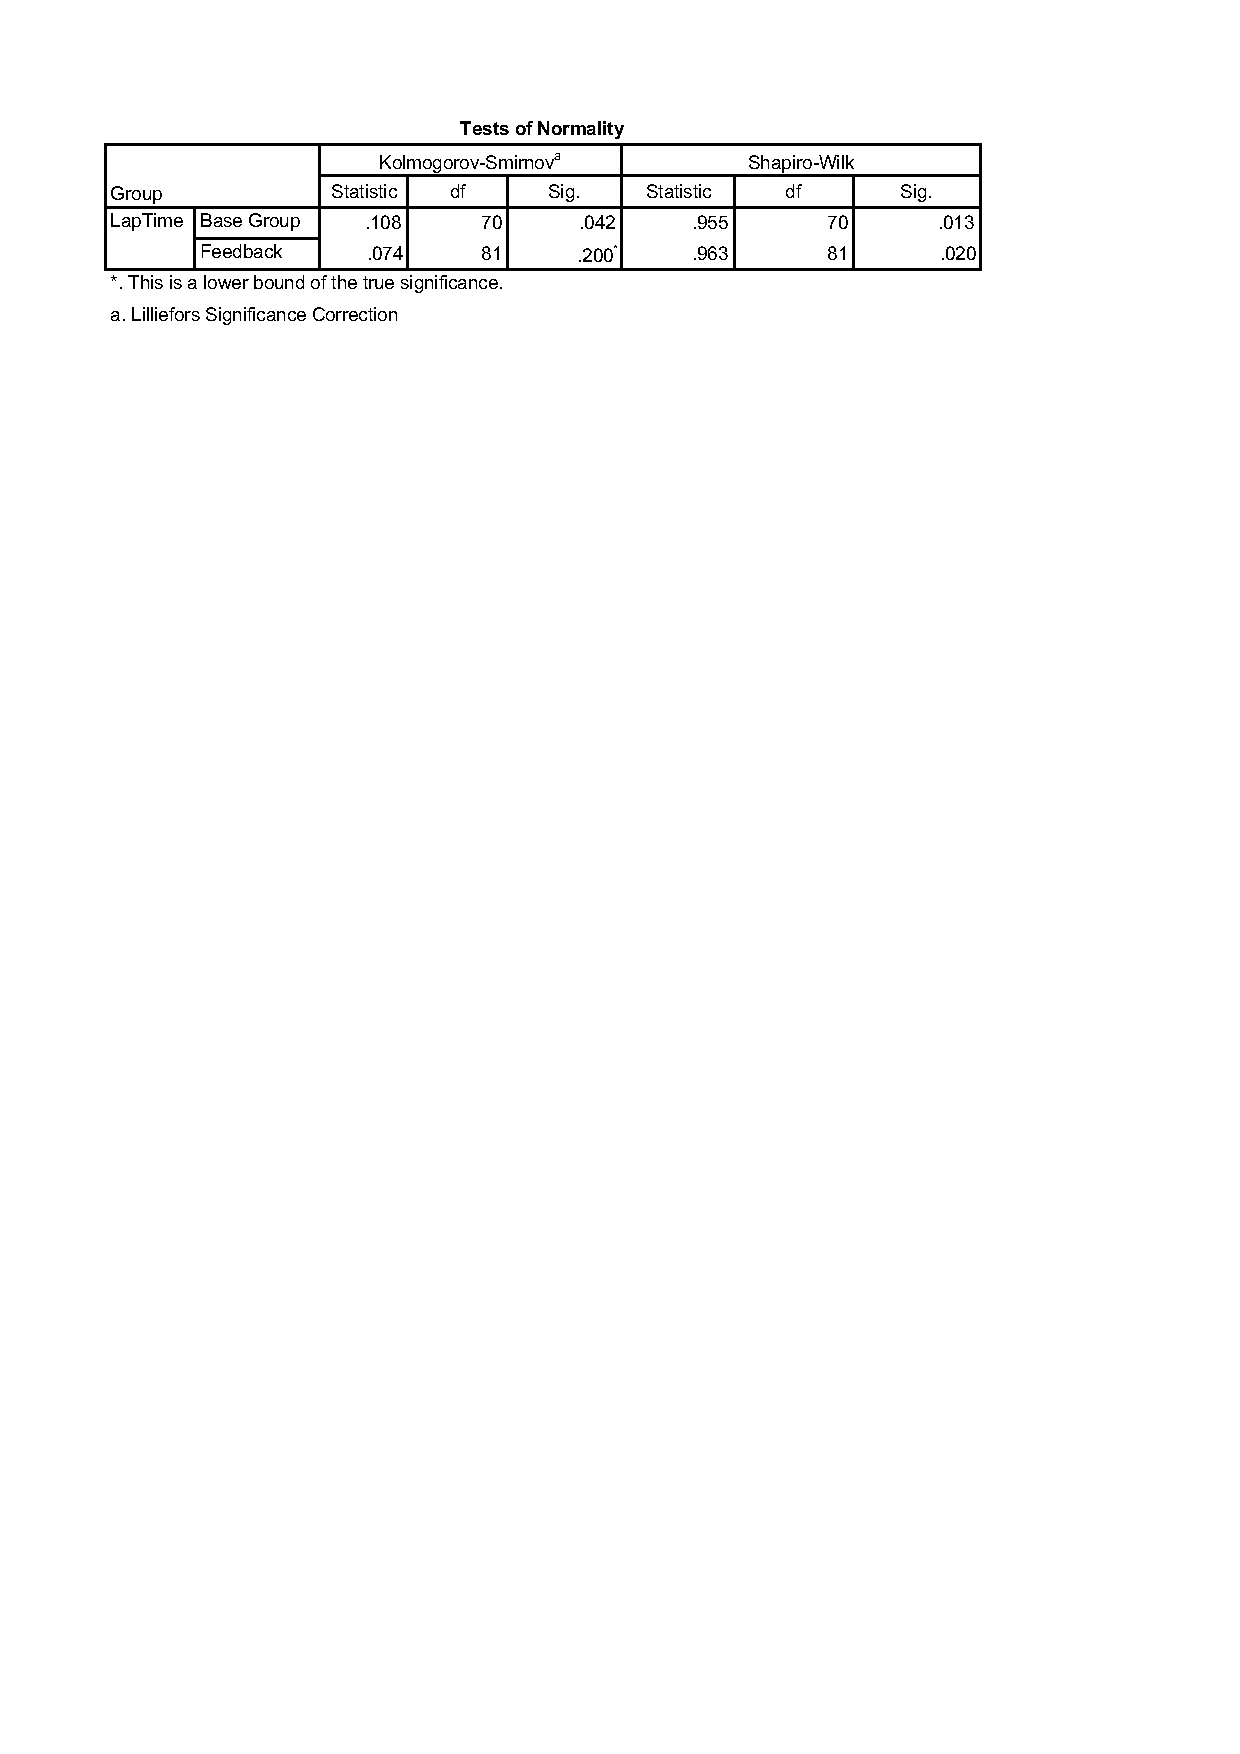
\includegraphics[width=\textwidth]{charts/shapiroWilkResults.pdf}
	\caption[Shapiro Wilk]{Shapiro Wilk test results}
	\label{fig:chart-shapiroWilk}
\end{figure}

The same data was checked for similar distribution across groups using the Independent Samples Kolmogorow-Smimov Test which resulted in accepting the null hypothesis stating the groups' lap times share the same distribution.

\begin{figure}[!htb]
	\centering
	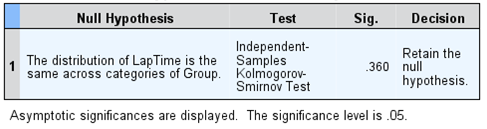
\includegraphics[width=\textwidth]{images/KolmogorowSmimov.png}
	\caption[Kolmogorow Smimov Test]{Kolmogorow Smimov test result}
	\label{fig:chart-KolmogorowSmimov}
\end{figure}

Having established both groups' lap times share the same distribution during the first session the Mann-Whitney Test to determine any differences between the groups before the feedback system is introduced. The test results show a p value of 0.057 resulting in no statistical difference between the groups at the start of the sessions.

\begin{figure}[!htb]
	\centering
	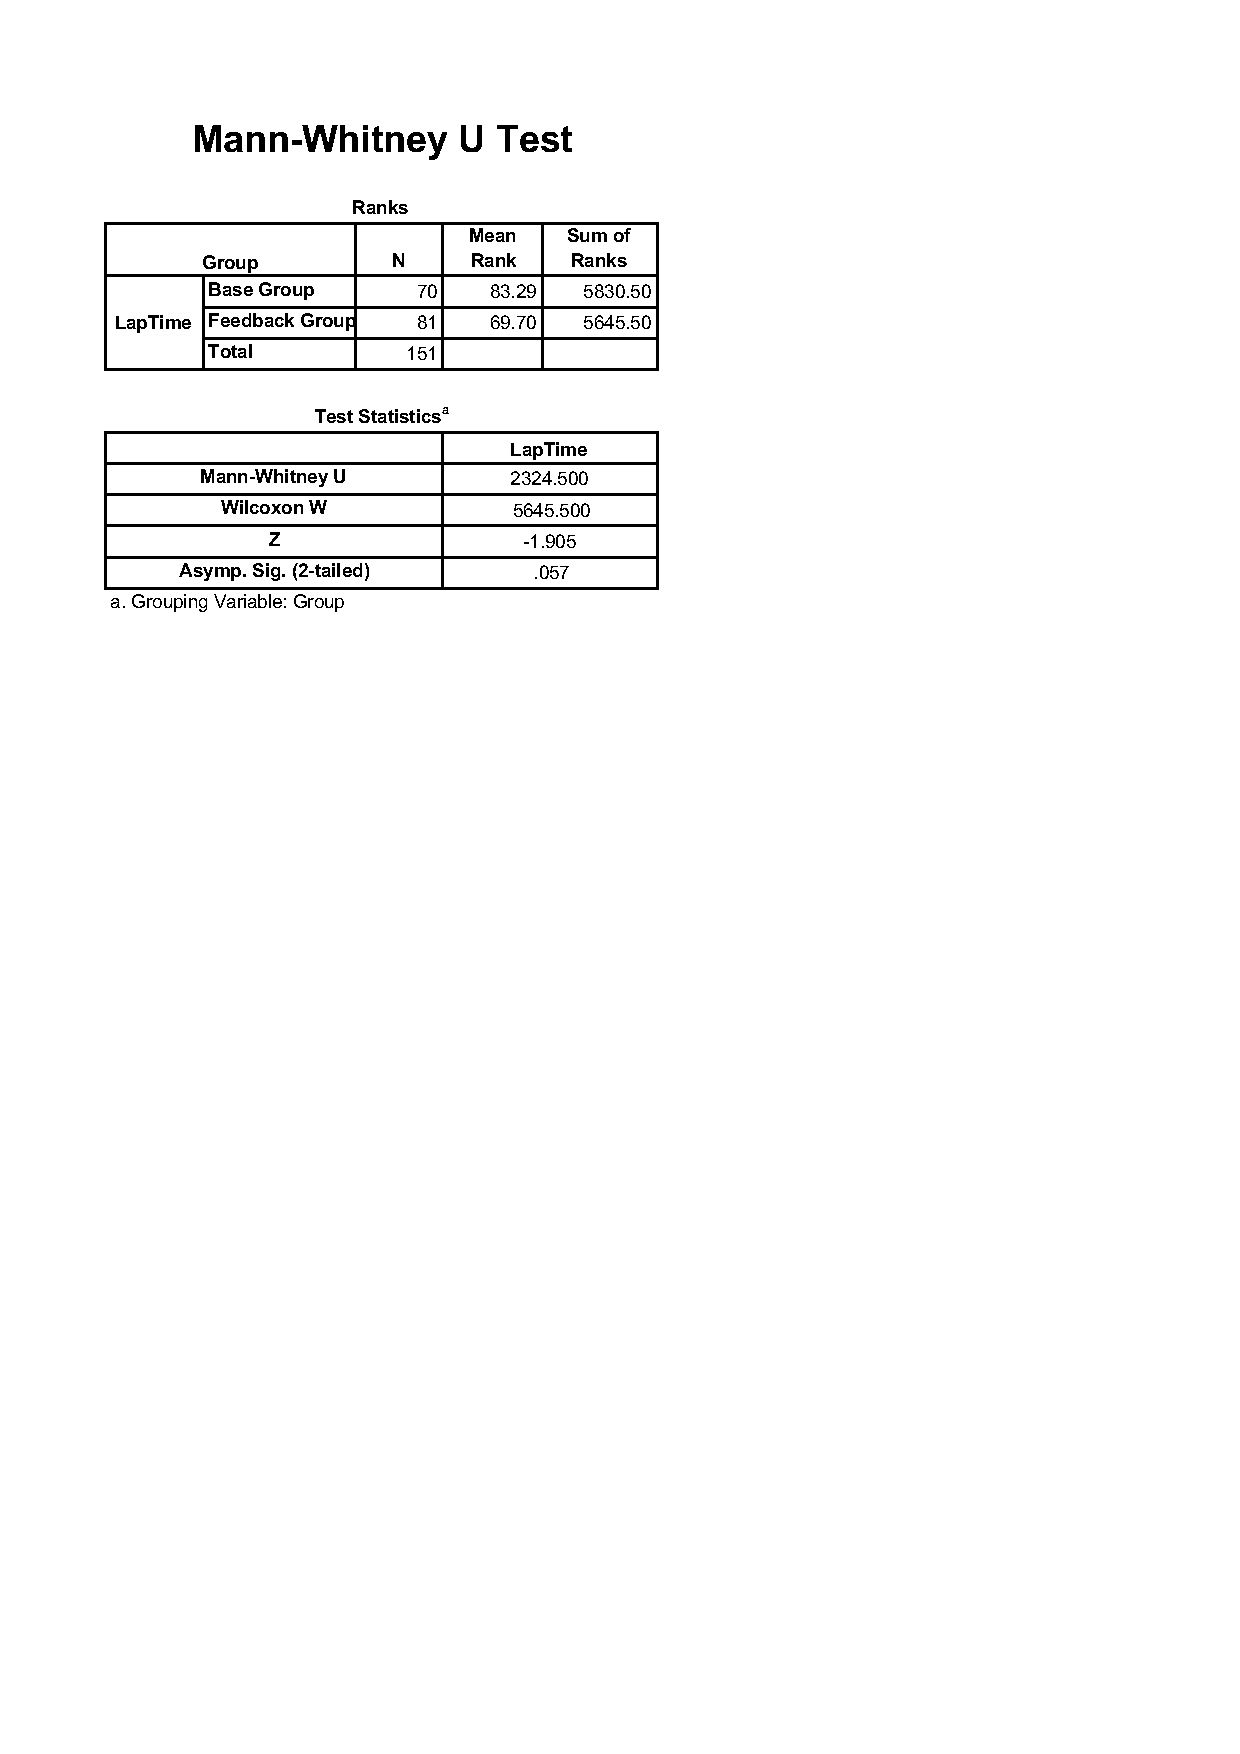
\includegraphics[width=\textwidth]{charts/Mann-Whitney.pdf}
	\caption[Mann-Whitney]{Mann-Whitney test result}
	\label{fig:chart-KolmogorowSmimov}
\end{figure}
